


%kerrotaan mikä on progressio ominaisuus. ja sitten kerrotaan minkälaiseksi se ominaisuus halutaan

%ominaisuus nimeltä tuntuu oudolta
Sovelluksessa on ominaisuus nimeltä Progressio. Ominaisuus antaa käyttäjälle mahdollisuuden seurata jotain mitattavaa arvoa, ja nähdä sen seurantaa kaavasta.
Arvoja voidaan myös käyttää raportissa.
%
Tällä hetkellä ominaisuus tukee vain yhtä mitattavaa arvoa.
Ominaisuutta haluttiin muuttaa siten että käyttäjälle voi antaa useamman mitattavan arvon. 
Tämän tekeminen vaatii käyttäjän skeeman muuntamista ja progressio sivun käyttöliittymän muuntamista.
\medskip






\subsection*{Kättäjä skeeman päivitys}

%schema skeema?=?

käyttäjän skeemassa on kenttä measurableThing joka on merkkijono mitattavan asian nimestä.
Tämän muuntaminen listaksi, johon voidaan lisätä useampi mitattava arvoja tuo ongelmia, sillä aktiiviset käyttäjät pitää migratoida käyttämään uutta käyttäjä skeemaa. 
Lisäksi pitää muokata rajapintoja ja käyttäjien muokkaamis- ja luomis- työkaluja.
\medskip


% jotain enemmän schemasta

Käyttäjän skeeman päivitys yksittäisestä measurableThing merkkijonosta measurableThings listaan vaatii töitä.
Käyttäjä mutaatio funktioiden toimintaa pitää muokata, sillä luodaan uusi kenttä ja poistetaan vanha.
Pitää myös etsiä kaikki kohdat, jossa measurableThing kenttää käytetään, ettei johda "cannot read properties of undefined"{} virheisiin.
käyttäjien muokkausta ja luontia pitää muokata siten että voimme lisätä ja poistaa mitattavia arvoja measurableThings listasta.
Rajapinnat ovat myös tyypitetty, joten niiden muuntaminen yhteensopivaksi on oleellista.
\medskip

% vähän jotain user migraatio funktiosta

Kaikki aktiiviset käyttäjät pitää myös muuttaa käyttämään uutta käyttäjä skeemaa.
Tämän voi toteuttaa funktiolla, joka käy kaikki käyttäjät läpi, luo niille measurableThings kentän ja siirtää alkuperäisen "measurableThing"{} mitattavan arvon listaan.
Tällaiset "migraatio funktiot"{} tuovat omat ongelmansa, sillä muokkaamme jokaista käyttäjää, ja jos muokkaaminen ei onnistu kaikilla aktiivisilla käyttäjille voi ilmentyä ongelmia.
Funktion pitää olla luotettava ja sellainen että se toimii ensimmäisellä kerralla.
\medskip




\subsection*{Käyttöliittymä}

%pitäskö olla tekstiä ennen kuvaa. ainakaan opparissa näin ei saa olla.

%mahdollisesti ota pienemmästä browser ikkunasta kun nyt on liian scuffed

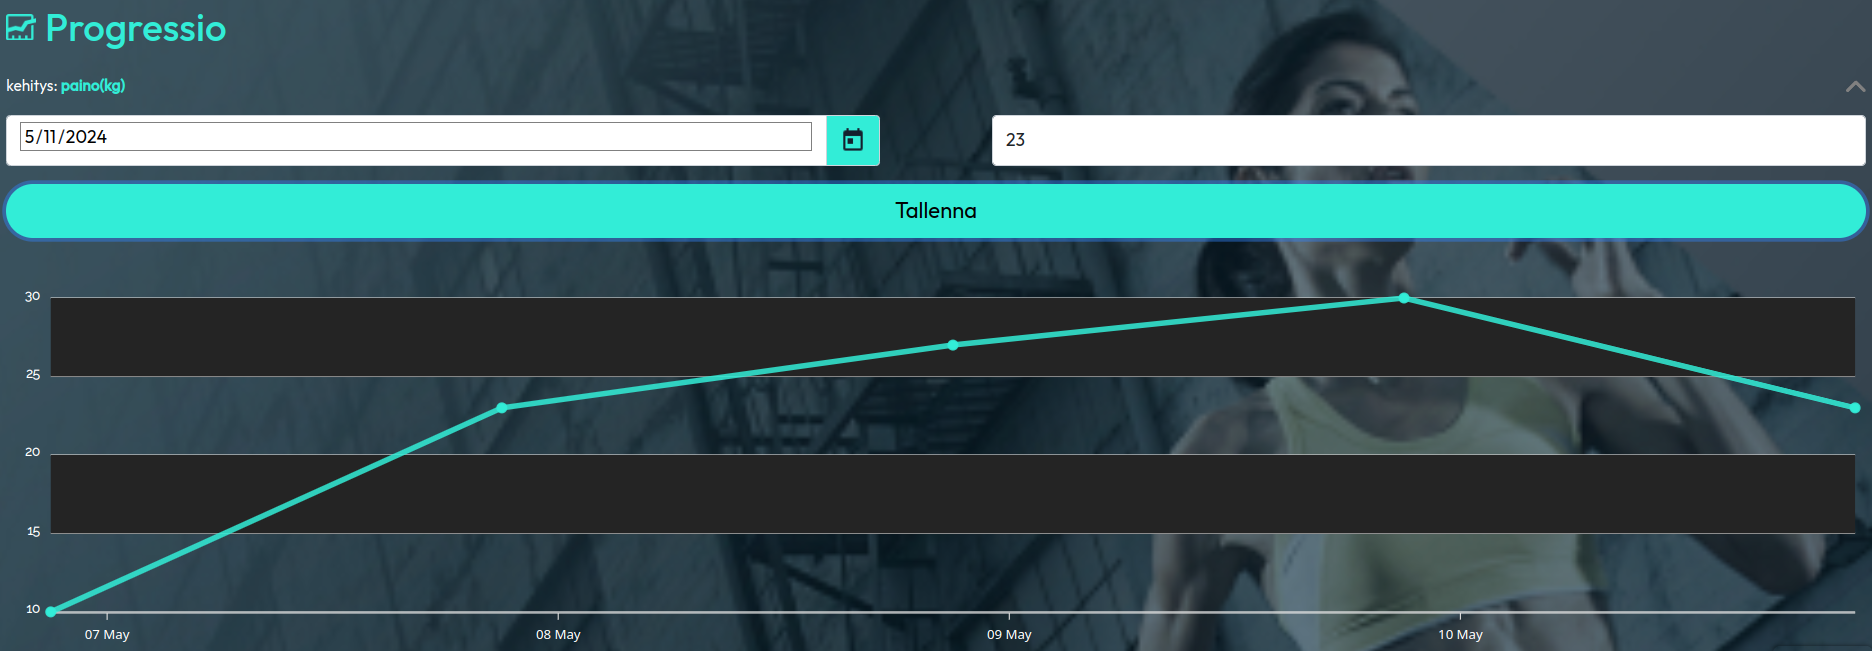
\includegraphics[width= 15cm]{src/public/progressiosingle.png} \\
starttaamo progressio sivu alussa
\medskip

%jotain tekstiä kuvasta 
Kuvassa näkyy nykyinen progressio ominaisuus. Käyttäjä voi valita päivän ja tallentaa arvon sille päivälle
vasemmassa reunassa näkyy "kehitys: paino(kg)"{} tämä on seuranta arvo, joka on annettu käyttäjälle, kun se on luotu.
Alempana on kaavio, josta käyttäjä voi nähdä seurattavan arvon kehittymistä. 
\medskip


% uusiks
Liittymästä käyttäjä voi tallentaa vain yhden seurattavan arvon. 
Kaavaa pitää muokata siten, että siitä voi nähdä kaikki seurattavat arvot.
Kaava käyttää React-apex-charts kirjastoa, joka tukee useamman viivan kaavion lisäämisen.
\medskip



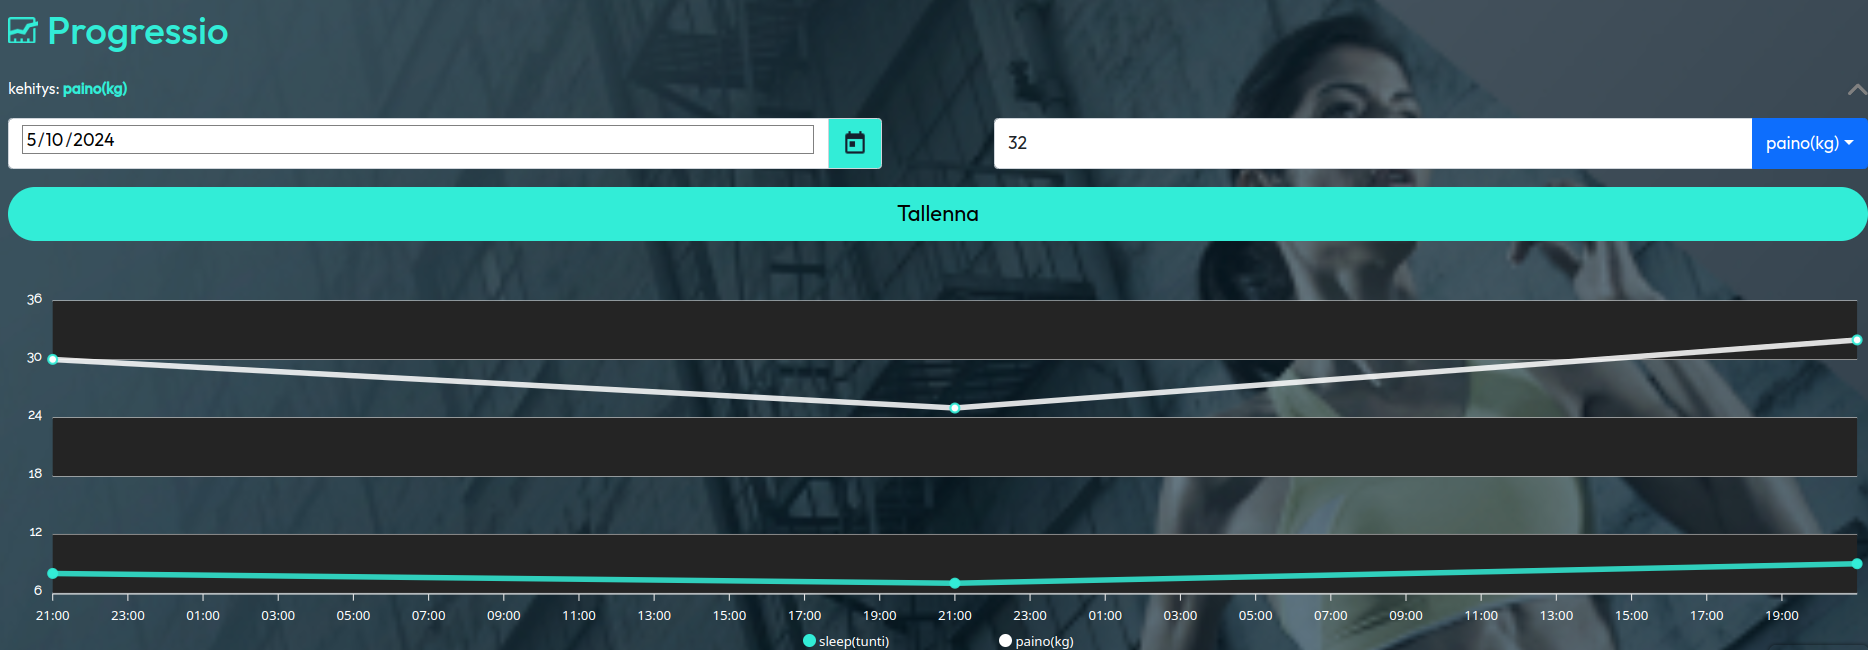
\includegraphics[width= 15cm]{src/public/progressmulti.png} \\
starttaamo progressio sivu ominaisuuden lisättyä
\medskip


Lisäsin myös laskuvalikon syöttökentän oikealle puolelle josta käyttäjä voi valita mitä mitattavaa hän haluaa tallentaa.

\iffalse

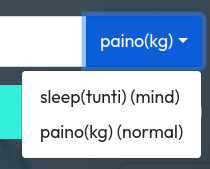
\includegraphics[width= 8cm]{src/public/progressselect.png} \\
mitattavien progressio arvojen laskuvalikko.
\medskip

laskuvalikon avautua käyttäjä voi valita mitä mitattavaa hän haluaa päivittää
\medskip

\fi




\subsection*{yhteenveto}
%lisää jotain tekstiä

React-apex-charts kirjastolla oli helpot työkalut kaavan muokkaamiseen, joten uuden datan lisääminen kaavioon oli helppoa.
User migraatio funktio oli toiminut oikein ja kaikki käyttäjät olivat saaneet ominaisuuden sen käyttöön ottamisen jälkeen.
Emme varmuuskopioinut käyttäjä tietoja ennen migraatiota, vaikka se olisi pitänyt tehdä. Näin ei olisi tullut ongelmaa jos migraatio funktio ei olisi toiminut.
Skeeman päivitys oli kaikista työläisin osa sillä rajapintojen vaihtaminen vaati paljon manuaalista työtä.
Muokkasin myös raportin luontia että se olisi yhteensopiva uuden ominaisuuden kanssa.




